\documentclass[a4paper,11pt,oneside]{book}  %bylo report
\usepackage[margin=0.75in]{geometry}
\usepackage[utf8]{inputenc} %ISO-8859-2 
\usepackage[polish]{babel} 
%\usepackage{times} 
\usepackage[T1]{fontenc} 
\usepackage[MeX]{polski} 
\usepackage[pdftex]{graphicx} 
\usepackage{pdfpages} 
\usepackage{fancyhdr} %numery stron po zewnętrznej 
\usepackage{wrapfig}
\usepackage[colorlinks=true,bookmarksopen,plainpages=false,urlcolor=blue,citecolor=black,filecolor=black,linkcolor=black,,unicode]{hyperref} 
\usepackage{titlesec} 
\usepackage{booktabs}
\usepackage{attachfile}
\usepackage{appendix}
\usepackage{listings}
\usepackage{tikz}
\usetikzlibrary{shapes,arrows,fit} %use shapes library if you need ellipse
\title{Sprawozdanie z projektu SPEKTROP\\ Blok elektroniki spektrometru obrazującego \\[10pt] \large{Creotech Instruments S.A.} \\ \large{Centrum Badań Kosmicznych}}
%\author{Piotr Zdunek}

\usepackage{newunicodechar}
\newunicodechar{fi}{fi}
\usepackage{courier}
\usepackage{listings}
\usepackage{float}
\pdfminorversion=5 
\pdfcompresslevel=9
\pdfobjcompresslevel=2
\usepackage{multirow}
\usepackage{url}
\usepackage{graphics}
\usepackage[section]{placeins}
\usepackage{hyperref}


\begin{document}
%\maketitle 
%
%\begin{table}[h]
%  \centering
%  \begin{tabular}{| c | c | c |}
%    \cline{1-3}  \textbf{Skład zespołu} & \textbf{Przedmiot} & \textbf{Data} \\
%   \hline
% 	Piotr Zdunek 	& \multirow{2}{*}{ Metody i~systemy pomiarowe wielkiej częstotliwości} & \multirow{2}{*}{07.04.2014} \\[5pt]
% 	Paweł Gontarek & & \\
%   \hline
%   \textbf{Prowadzący} 		& \textbf{Tytuł ćwiczenia}	&	\textbf{Numer stanowiska} \\
%   \hline
%   dr~inż. Wojciech Wiatr	&	Pomiar parametrów materiałowych metodą rezonansową	&	2			\\
%   \hline
%  \end{tabular}
%    \label{tab:tytulowa}
%\end{table}





\maketitle


\lstdefinestyle{custom}{
  belowcaptionskip=1\baselineskip,
  breaklines=true,
  frame=L,
  xleftmargin=\parindent,
  language=Matlab,
  showstringspaces=false,
  basicstyle=\footnotesize\ttfamily,
  keywordstyle=\bfseries\color{green!40!black},
  commentstyle=\itshape\color{purple!40!black},
  identifierstyle=\color{blue},
  stringstyle=\color{orange},
}

\lstset{escapechar=@,style=custom}

%\tableofcontents
%\newpage	
\chapter{Wstęp} 
Poniższy dokument jest sprawozdaniem z projektu bloku elektroniki spektrometru obrazującego SPEKTROP zaprojektowanego przez Creotech Instruments S.A. na zlecenie Centrum Badań Kosmicznych. Zawarto w nim specyfikację systemu, sposób działania oraz opis zastosowanych rozwiązań sprzętowych i programowych. 

Projekt SPEKTROP jest systemem kamery spektralnej, umieszczonej na samolocie bądź UAV\footnote{UAV - Unmanned Aerial Vehicle} pozwalającym na rejestrację obrazu lądu jednocześnie w wielu długościach fali.
Takie rozwiązanie pozwala na analizę powierzchni różnych rodzajów obszarów jak lasy, jeziora, pola uprawne. Czy analizę możliwości wystąpienia złóż.

\begin{figure}[htp]
	\centering
	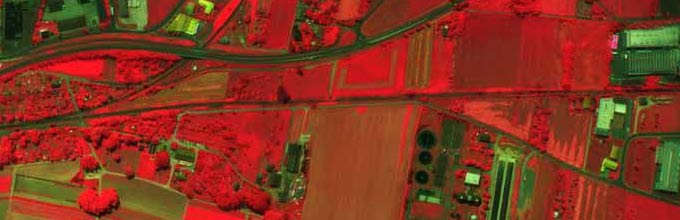
\includegraphics[width=12cm]{spektrop_ex.jpg}
	\caption{Przykładowy obraz z kamery spektralnej\cite{SPEC_PHOTO}}
	\label{fig:EX_PHOTO}
\end{figure}


Sercem zaprojektowanego urządzenia jest układ SoC Zynq Z7045, który łączy w sobie układ FPGA Kintex 7 oraz dwurdzeniowy procesor ARM Cortex-A8. System pozwala na rejestrację danych z czujnika CMV4000 z maksymalną prędkością 100 FPS przy minimalnym czasie ekspozycji wynoszącym $\sim$ 10 ms.Ponadto system umożliwia rejestrację parametrów lotu niezależnie od akwizycji obrazu oraz z możliwością przyporządkowania danych do poszczególnych klatek. Dzięki czemu możliwa jest późniejsz analiza zebranych danych. Zebrane dane są zapisywane na dysku/ach HDD poprzez interfejs SATA zaimplementowanym w logice FPGA przy pomocy transceiverów GTX.

Sterowanie i komunikacja z systemem odbywa się poprzez interfejs Ethernet przy pomocy dedykowanej aplikacji działającej pod systemem Linux. 


\chapter{Specyfikacja}

\section{Czujnik CMOS}
\begin{itemize}
	\item Detektor: CMV4000 \cite{CMV4000} albo CIS 1910F \cite{CIS}.
	\item Tryby pracy czujnika:
		\begin{itemize}
			\item Podstawowy: czas ekspozycji (EXP\footnote{EXP - Exposure}) 1-10 ms, 100 FPS\footnote{FPS -Frames Per Second}
			\item Manualny:	dowolnie długi czas ekspozycji z mniejszą ilością FPS (np. 5-10 FPS przy EXP $\sim$ 1-2 ms
		\end{itemize}

	\item Rozdzielczość bitowa - 16 bit/piksel, ENOB\footnote{ENOB - Effective Number of Bits}:8-9 bitów
	\item Zakres temperatury pracy: $-10^{o}C \div +50^{o}C$

\end{itemize}

\section{Platforma sprzętowa}
\begin{itemize}
\item Xilinx Zynq Evaluation Board ZC706 \cite{ZC706}
\end{itemize}

\section{System rejestracji parametrów lotu}

\begin{itemize}
\item rejestracja parametrów lotu na podstawie systemów GPS oraz IMU\footnote{IMU - Internal Management Unit} z zapewnieniem synchronizacji czasowej względem akwizycji klatek i niezależnie 
	\begin{itemize}
	\item minimalny okres zapisu parametrów - 0.1 s
	\end{itemize}
\item zapis czasu pomiaru (timestamp) i czasu akwizycji parametrów lotu
\item nośnikiem danych jest dysk twardy 
%(SSD\footnote{SSD - Solid State Drive}/HDD\footnote{HDD - Hard Disk Drive}) z interfejsem SATA,
(SSD/HDD) z interfejsem SATA, zapis odbywa się przy pomocy interfejsu GTX
\end{itemize}



\section{Tryby pracy}

\begin{itemize}
\item Ręczny - ustawiany przez operatora przy pomocy komputera PC (operator leci w samolocie)
\item Autonomiczny - posiadający następujące funkcje: 
	\begin{itemize}
		\item wyliczanie ekspozycji i częstotliwości akwizycji klatek na podstawie parametrów lotu dostarczanych przez systemy sterujące samolotu/UAV
		\item sprawdzanie poprawności ekspozycji
		\item możliwość wyzwalania pomiarów na podstawie osiągnięcia pozycji wskazanej przez GPS
	\end{itemize}
	
\end{itemize}

\section{Wymagania elektryczne}

Napięcie zasilania 24 V albo 12 V. 

\section{Wymagania mechaniczne}

Wymiary PCB: 85 mm x 160 mm. 


\section{Proponowany schemat funkcjonalny systemu}

\begin{figure}[!h]
	\centering
	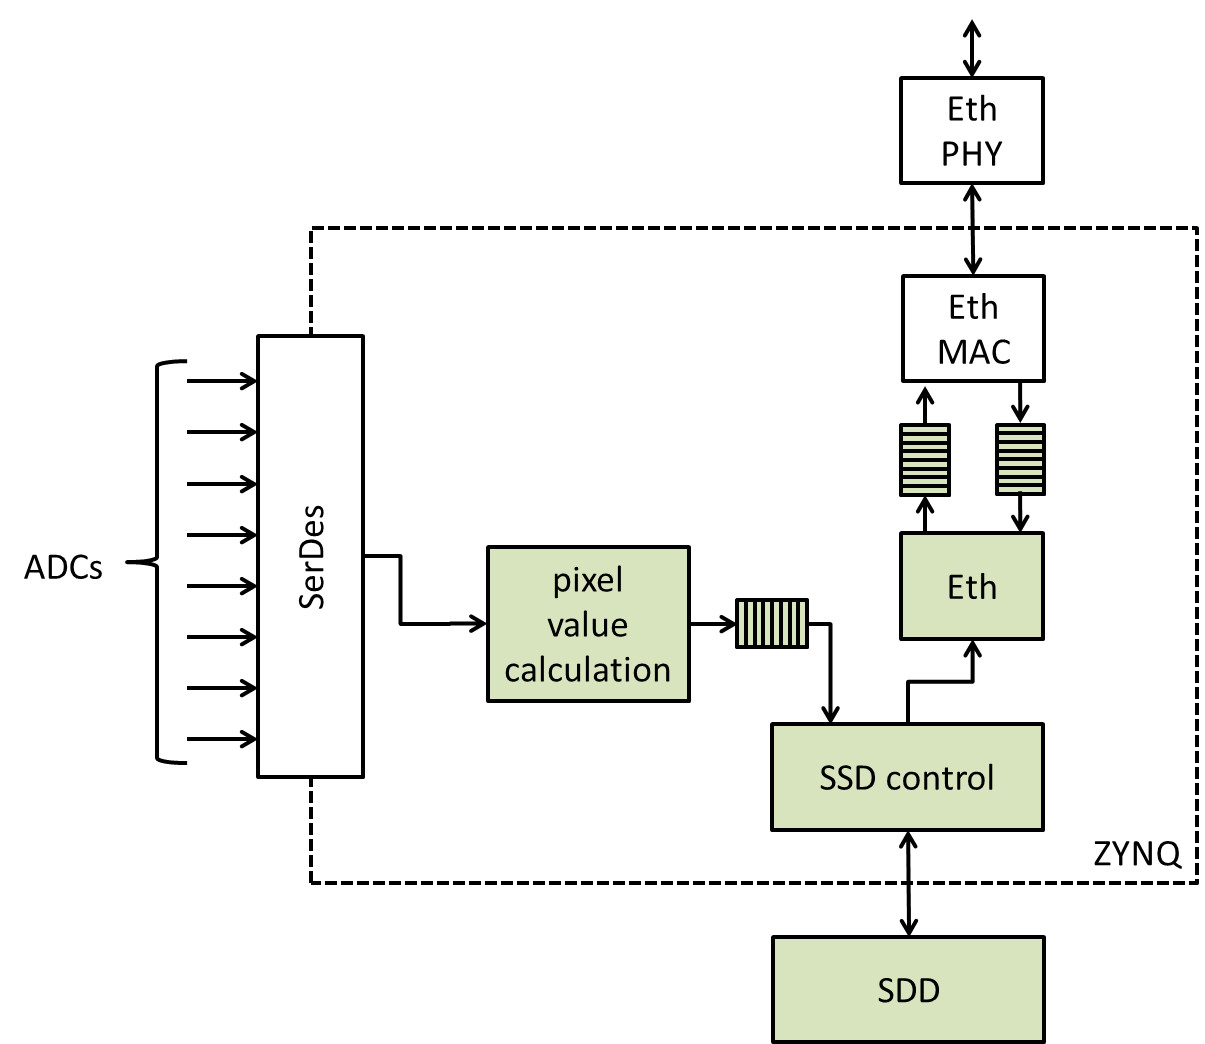
\includegraphics[width=12cm]{schemat_cbk.jpg}
	\caption{Schemat blokowy systemu}
	\label{fig:SYS}
\end{figure}


%\section{Założenia}

\chapter{Koncepcja realizacji}

Poniższy rozdział opisuje koncepcję realizacji bloku elektroniki projektu SPEKTROP. Rysunek [\ref{fig:OVER}] przedstawia główne elementy systemu: 
\begin{itemize}
	\item płytę ewaluacyjną ZC706
	\item czujnik CMOSIS MV4000
	\item interfejs SATA
	\item interfejs Ethernet
	\item połączenie z systemem GPS i IMU
\end{itemize}
\begin{figure}[!h]
	\centering
	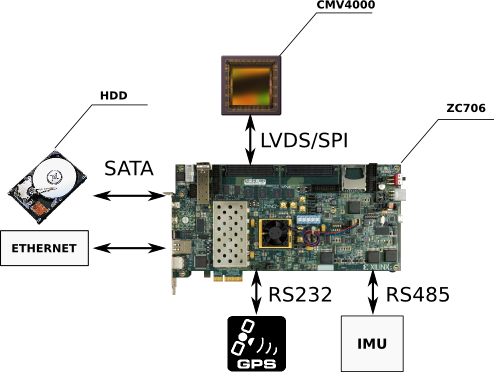
\includegraphics[width=12cm]{OVER2.png}
	\caption{Główne elementy systemu}
	\label{fig:OVER}
\end{figure}



Czujnik CMV4000 będzie połączony z modułem ZC706 poprzez złącze FMC. Zebrane dane będą przesłane poprzez interfejs SATA. Do systemu jest równiez dołączone IMU UAV/samolotu oraz moduł GPS. System jest sterowany poprzez interfejs Ethernet. 


\chapter{Realizacja}
Rysunek [\ref{fig:SCHEMAT}] zawiera schemat blokowy systemu. System składa się z modułu ewaluacyjnego układu Zynq ZC706, oraz z modułu FMC z czujnikiem CMOSIS CMV4000.
%\subsection{Wstęp}

\begin{figure}[!h]
	\centering
	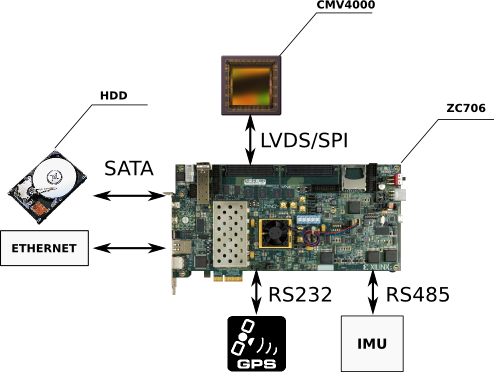
\includegraphics[width=12cm]{OVER2.png}
	\caption{Główne elementy systemu}
	\label{fig:OVER}
\end{figure}

\section{Platforma sprzętowa}
System oparty jest o moduł ewaluacyjny ZC706 posiadjący wszystkie podstawowe komponenty sprzętowe potrzebne do realizacji zaawansowanych systemów przetwarzania.

\begin{figure}[H]
	\centering
	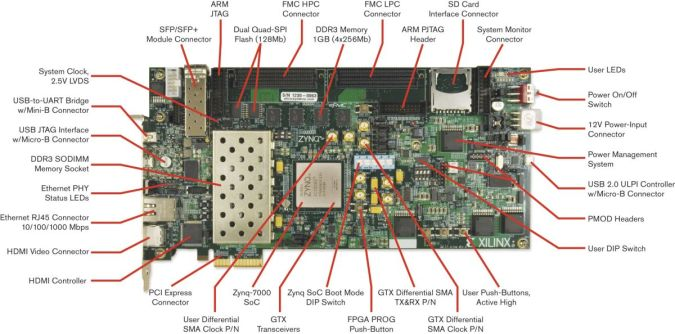
\includegraphics[width=12cm]{zc706-base-board.jpg}
	\caption{Elementy płyty ewaluacyjnej ZC706}
	\label{fig:ZC706}
\end{figure}

Moduł posiada następujące komponenty:
\begin{itemize}
\item Układ SoC
	\begin{itemize}
	\item Zynq-7000 XC7Z045 FFG900 
	\end{itemize}
	
\item Konfiguracja
	\begin{itemize}
	\item 2X16MB Quad SPI Flash
	\item SDIO 
	\item PC4 i JTAG 
	\end{itemize}

\item Pamięć
	\begin{itemize}
	\item DDR3 Component Memory 1GB (PS)
	\item DDR3 SODIM Memory 1GB (PL)
	\item 2X16MB Quad SPI Flash
	\item IIC - 1 KB EEPROM
	\end{itemize}
	
\item Interfejsy komunikacyjne
	\begin{itemize}
	\item PCIe Gen2x4
	\item SFP+ and SMA Pairs
	\item GigE RGMII Ethernet (PS)
	\item 1 CAN with Wake on CAN (PS)
	\item USB OTG 1 (PS) - Host USB
	\item IIC Bus Headers/HUB (PS)
	\item USB UART (PS)
	\end{itemize}

\item Komponenty wideo
	\begin{itemize}
	\item HDMI 8 color RGB 4.4.4 1080P-60 OUT
	\item HDMI IN 8 color RGB 4.4.4
	\end{itemize}
	
\item Złącza we/wy
	\begin{itemize}
	\item FMC LPC 
	\item FMC HPC
	\item Pmod dualny i pojedynczy
	\item Dostęp do I2C
	\item USB OTG 1 (PS) - Host USB
	\item IIC Bus Headers/HUB (PS)
	\item USB UART (PS)
	\end{itemize}
	
\item Sygnały zegarowe
	\begin{itemize}
	\item 33MHz Zegar systemowy
	\item 200MHz PL Oscylator
	\item złącza SMA dla zewnętrznych sygnałów zegarowych
	\item referencyjne do GTX 
	\item OBSAI/CPRI – SFP+ 
	\item EXT Config CLK
	\end{itemize}

\item Sterowanie
	\begin{itemize}
	\item 2 User Push Buttons/Dip Switch, 2 User LEDs
	\item 3 User Push Buttons, 2 User Switches, 8 User LEDs
	\item IIC access to 8 I/O
	\item IIC access to a WTClock
	\end{itemize}

\item Zasilanie
	\begin{itemize}
	\item 12 V 
	\item możliwość pomiaru prądu linii zasilających
	\end{itemize}
\end{itemize}

\section{Realizacja programowa}

\section{Akwizycja danych z czujnika}

\section{System rejestracji parametrów lotu}

\section{Zapis danych}

\subsection{Interfejs SATA}



\chapter{Podsumowanie}





\begin{thebibliography}{9}
\bibitem{SPEC} Specyfikacja wymagań modułu odczytowgeo układu UFXC - Firmware
\bibitem{ZC706} Xilinx ZC706 Evaluation Board \url{http://www.xilinx.com/products/boards-and-kits/EK-Z7-ZC706-G.htm}
\bibitem{CMV4000} CMOSIS CMV4000 Sensor \url{http://www.cmosis.com/products/standard_products/cmv4000}
\bibitem{CIS} CIS 1910F Sensor
\bibitem{SPEC_PHOTO} \url{http://www.steadidrone.eu/uav-hexacopter-h6x-for-precise-agriculture/}
\end{thebibliography}
\end{document}
